\documentclass[journal]{IEEEtran}
\usepackage[english]{babel}

\usepackage{amssymb, amsmath} %Paquetes matemáticos de la American Mathematical 
\usepackage[utf8]{inputenc}
\usepackage{graphicx}
\usepackage{float}
\usepackage{hyperref}
\usepackage{listings}
\usepackage{xcolor}

\definecolor{codegreen}{rgb}{0,0.6,0}
\definecolor{codegray}{rgb}{0.5,0.5,0.5}
\definecolor{codepurple}{rgb}{0.58,0,0.82}
\definecolor{backcolour}{rgb}{0.95,0.95,0.92}
% Definicio de estilo para el codigo fuente que se cita
\lstdefinestyle{mystyle}{
    backgroundcolor=\color{backcolour},   
    commentstyle=\color{codegreen},
    keywordstyle=\color{magenta},
    numberstyle=\tiny\color{codegray},
    stringstyle=\color{codepurple},
    basicstyle=\ttfamily\footnotesize,
    breakatwhitespace=false,         
    breaklines=true,                 
    captionpos=b,                    
    keepspaces=true,
    numbers=left,                    
    numbersep=5pt,                  
    showspaces=false,                
    showstringspaces=false,
    showtabs=false,                  
    tabsize=2,
}
\lstset{style=mystyle}

\renewcommand{\lstlistingname}{Código}

\ifCLASSINFOpdf

\else

\fi
\begin{document}

\title{Ejercicio 2 - tema 7 \\ Almacenamiento en data files}
%
\author{Vicente Romero Andrade}

\markboth{Ejercicio 2 - tema 7 Almacenamiento en data files, Julio~2021}%
{Shell \MakeLowercase{\textit{et al.}}: }
% The only time the second header will appear is for the odd numbered pages

\maketitle


\IEEEpeerreviewmaketitle

\section{Objetivo}
% The very first letter is a 2 line initial drop letter followed

\IEEEPARstart{E}{l} objetivo es poner en práctica las tareas de administración 
que permitan el almacenamiento de datos de una tabla en un tablespace y data file 
específico configurado previamente

\section{Desarrollo}
\subsection{sentencias}
\begin{lstlisting}[language=sql, caption=s-00-datafile.sql,label={lst:codigo1}]
  whenever sqlerror exit rollback
  set serveroutput on
  connect sys/system2 as sysdba
  --A
  SELECT
    FILE_NAME,
    FILE_ID,
    TRUNC((BYTES/(1024*1024)),2) SIZE_MB
  FROM DBA_DATA_FILES WHERE TABLESPACE_NAME ='STORE_TBS_MULTIPLE';
  --B
  SELECT
         TRUNC((SUM(DF.BYTES)-NVL(SUM(S.BYTES),0))/(1024*1024),2) MB_LIBRES,
         (SUM(DF.BLOCKS)-NVL(SUM(S.BLOCKS),0)) BLOQUES_DISPONIBLES
  FROM DBA_DATA_FILES DF
      LEFT JOIN DBA_SEGMENTS S
          ON S.TABLESPACE_NAME = DF.TABLESPACE_NAME
  WHERE DF.TABLESPACE_NAME='STORE_TBS_MULTIPLE';
  --C
  --CREATE USER VRA_TBS_MULTIPLE IDENTIFIED BY VRA_TBS_MULTIPLE 
    --quota unlimited on store_tbs_multiple 
    --default tablespace store_tbs_multiple;
  --D
  declare
    v_count number;
    v_username varchar2(30) := 'VRA_TBS_MULTIPLE';
    v_table varchar2(30) := 'VRA_TBS_MULTIPLE';
  begin
    --Verificar si la table existe
    select count(*) into v_count
    from all_tables
    where table_name = v_table
    and owner = v_username;
  
    if v_count > 0 then
      execute immediate 'drop table '||v_username||'.'||v_table;
    end if;
    execute immediate 'create table '||v_username||'.'||v_table||' (
      str char(1024 byte)
    ) segment creation immediate';
  end;
  /
  --E
  SELECT DF.FILE_NAME,
         DF.FILE_ID,
         COUNT(DE.SEGMENT_NAME) NUMERO_EXTENSIONES,
         SUM(DE.BYTES/(1024*1024)) TOTAL_MB,
         SUM(DE.BLOCKS) BLOQUES_RESERVADOS
      FROM DBA_SEGMENTS DS
  JOIN DBA_DATA_FILES DF
      ON DS.HEADER_FILE = DF.FILE_ID
  JOIN DBA_DATA_FILES DF
      ON DS.HEADER_FILE = DF.FILE_ID
  JOIN DBA_EXTENTS DE
      ON DS.SEGMENT_NAME = DE.SEGMENT_NAME
  WHERE DS.SEGMENT_NAME like '%VRA_TBS_MULTIPLE%'
  GROUP BY DF.FILE_NAME, DF.FILE_ID;
  --F
  declare
    v_count number := 0;
  begin
    while v_count < 512 loop
    insert into VRA_TBS_MULTIPLE.VRA_TBS_MULTIPLE(str) values('$');
    v_count := v_count + 1;
    end loop;
    commit;
  end;
  /
  --G
  SELECT DF.FILE_NAME,
         DF.FILE_ID,
         COUNT(DE.SEGMENT_NAME) NUMERO_EXTENSIONES,
         SUM(DE.BYTES/(1024*1024)) TOTAL_MB,
         SUM(DE.BLOCKS) BLOQUES_RESERVADOS
      FROM DBA_SEGMENTS DS
  JOIN DBA_DATA_FILES DF
      ON DS.HEADER_FILE = DF.FILE_ID
  JOIN DBA_DATA_FILES DF
      ON DS.HEADER_FILE = DF.FILE_ID
  JOIN DBA_EXTENTS DE
      ON DS.SEGMENT_NAME = DE.SEGMENT_NAME
  WHERE DS.SEGMENT_NAME like '%VRA_TBS_MULTIPLE%'
  GROUP BY DF.FILE_NAME, DF.FILE_ID;
  --H
  declare
    v_count number := 0;
  begin
    while v_count < 512*5 loop
    insert into VRA_TBS_MULTIPLE.VRA_TBS_MULTIPLE(str) values('$');
    v_count := v_count + 1;
    end loop;
    commit;
  end;
  /
  SELECT DF.FILE_NAME,
         DF.FILE_ID,
         COUNT(DE.SEGMENT_NAME) NUMERO_EXTENSIONES,
         SUM(DE.BYTES/(1024*1024)) TOTAL_MB,
         SUM(DE.BLOCKS) BLOQUES_RESERVADOS
      FROM DBA_SEGMENTS DS
  JOIN DBA_DATA_FILES DF
      ON DS.HEADER_FILE = DF.FILE_ID
  JOIN DBA_DATA_FILES DF
      ON DS.HEADER_FILE = DF.FILE_ID
  JOIN DBA_EXTENTS DE
      ON DS.SEGMENT_NAME = DE.SEGMENT_NAME
  WHERE DS.SEGMENT_NAME like '%VRA_TBS_MULTIPLE%'
  GROUP BY DF.FILE_NAME, DF.FILE_ID;
  --I
  SELECT
         TRUNC((SUM(DF.BYTES)-NVL(SUM(S.BYTES),0))/(1024*1024),2) MB_LIBRES,
         (SUM(DF.BLOCKS)-NVL(SUM(S.BLOCKS),0)) BLOQUES_DISPONIBLES
  FROM DBA_DATA_FILES DF
      LEFT JOIN DBA_SEGMENTS S
          ON S.TABLESPACE_NAME = DF.TABLESPACE_NAME
  WHERE DF.TABLESPACE_NAME='STORE_TBS_MULTIPLE';
  
  whenever sqlerror continue
\end{lstlisting}

\begin{figure}[H]
  \centering
  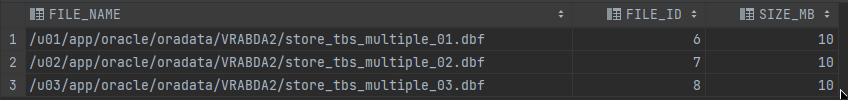
\includegraphics[scale=.25]{captura_a.png}
   \caption{Salida punto A}
   \label{fig:validador_1}
\end{figure}
\begin{figure}[H]
  \centering
  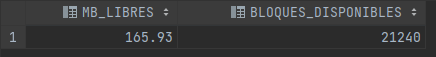
\includegraphics[scale=.50]{captura_4.png}
   \caption{Salida punto B}
   \label{fig:validador_2}
\end{figure}
\begin{figure}[H]
  \centering
  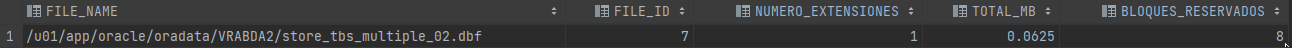
\includegraphics[scale=.19]{captura_1.png}
   \caption{Salida punto E}
   \label{fig:validador_3}
\end{figure}
\subsubsection{¿Qué data files se usaron para inicializar su segmento?}
Se uso /u03/app/oracle/oradata/VRABDA2/store\_tbs\_multiple\_02.dbf
\begin{figure}[H]
  \centering
  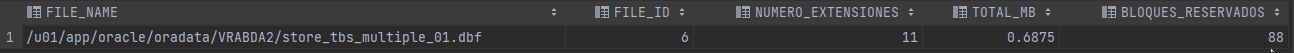
\includegraphics[scale=.19]{captura_2.png}
   \caption{Salida punto G}
   \label{fig:validador_4}
\end{figure}
\subsubsection{¿Qué diferencias se observan?}
El numero de bloques reservados y el total de MB usados
\begin{figure}[H]
  \centering
  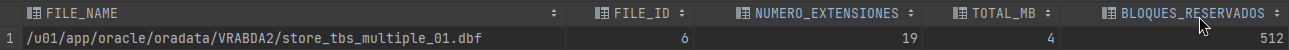
\includegraphics[scale=.19]{captura_3.png}
   \caption{Salida punto H}
   \label{fig:validador_5}
\end{figure}
\subsubsection{¿Qué diferencias se observan?} 
en el numero de extensiones, el total de MB y los blques
\subsubsection{¿Cuántas extensiones hasta el momento se han reservado?}
19
\subsubsection{¿Cuál es el espacio total reservado hasta el momento?}
4 MB
\subsubsection{¿Qué sucede con los demás data files que integran a este tablespace?}
Aun no se usan ya que aun hay espacio en el primer datafile
\begin{figure}[H]
  \centering
  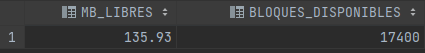
\includegraphics[scale=.35]{captura_5.png}
   \caption{Salida punto I}
   \label{fig:validador_6}
\end{figure}
\subsubsection{¿Qué diferencias se observan?} 
El numero de bloques y MB libres disminuyo
\section{Conclusiones}
Fue un ejercicio que demostro la forma de poder monitorear el espacio de almacenamiento 
que se va ocupando en una base de datos, este es ocupado en los datafiles y se distribuye de una 
forma secuencial.
\ifCLASSOPTIONcaptionsoff
  \newpage

\fi

\end{document}
